\subsubsection{Evaluation of $K\left( \epsilon \right) $ if the small $%
\epsilon $ approximation}\label{efftrappedfrac}

We can rewrite
\begin{equation}
I\left( \xi_{0}\right) =\frac{1}{\left( 1+\epsilon\right) }%
\int_{\xi_{0T}}^{\xi_{0}}\frac{d\xi_{0}^{\prime}}{\lambda_{2,-1,0}\left(
\xi_{0}^{\prime }\right) }
\end{equation}
with, for $\xi_{0}^{\prime}>\xi_{0T}$,
\begin{equation}
\lambda_{2,-1,0}\left( \xi_{0}^{\prime}\right) =\int_{0}^{2\pi}\frac
{d\theta}{2\pi}\frac{\xi^{\prime}}{\Psi\xi_{0}^{\prime}}
\end{equation}
where
\begin{equation}
\xi^{\prime}=\sqrt{1-\Psi\left( 1-\xi_{0}^{\prime2}\right) }
\end{equation}

In the limit $\epsilon\ll1$, we have
\begin{align}
\Psi & \equiv\frac{1+\epsilon}{1+\epsilon\cos\theta}  \nonumber \\
& =\left( 1+\epsilon\right) \left[ 1-\epsilon\cos\theta+\mathcal{O}\left(
\epsilon^{2}\right) \right]  \nonumber \\
& =1+\epsilon\left( 1-\cos\theta\right) +\mathcal{O}\left( \epsilon
^{3}\right)
\end{align}
so that
\begin{align*}
\xi^{\prime} & =\sqrt{1-\left[ 1+\epsilon\left( 1-\cos\theta\right) +%
\mathcal{O}\left( \epsilon^{2}\right) \right] \left( 1-\xi_{0}^{\prime
2}\right) } \\
& =\xi_{0}^{\prime}\sqrt{1-\epsilon\frac{\left( 1-\cos\theta\right) \left(
1-\xi_{0}^{\prime2}\right) }{\xi_{0}^{\prime2}}+\mathcal{O}\left(
\epsilon^{2}\right) }
\end{align*}

In fact, the series expansion of the square root must be kept to all orders
for the term in $\epsilon$, because the ratio $\epsilon/\xi_{0}^{\prime
2}\rightarrow1$ for $\xi_{0}^{\prime}\rightarrow\xi_{0T}$. This gives
\[
\xi^{\prime}=\xi_{0}^{\prime}\left\{ 1-\sum_{n=1}^{\infty}\frac{\left(
2n-2\right) !}{2^{2n-1}\left( n-1\right) !n!}\left[ \frac{\epsilon\left(
1-\cos\theta\right) \left( 1-\xi_{0}^{\prime2}\right) }{\xi_{0}^{\prime2}}%
\right] ^{n}+\mathcal{O}\left( \epsilon^{2}\right) \right\} 
\]
where we used
\begin{align}
\left( 1+x\right) ^{\alpha} & =1+\sum_{n=1}^{\infty}\frac{\alpha\left(
\alpha-1\right) \cdots\left( \alpha-n+1\right) }{n!}x^{n} \\
\left( 1+x\right) ^{1/2} & =1+\sum_{n=1}^{\infty}\frac{1}{2}\left( \frac{1}{2%
}-1\right) \cdots\left( \frac{1}{2}-n+1\right) \frac{x^{n}}{n!} \\
& =1+\frac{1}{2}x+\sum_{n=2}^{\infty}\frac{\left( -1\right) ^{n-1}}{2^{n}}%
\left( 1\right) \left( 3\right) \cdots\left( 2n-3\right) \frac{x^{n}}{n!} \\
& =1+\frac{1}{2}x+\sum_{n=2}^{\infty}\frac{\left( -1\right) ^{n-1}\left(
2n-3\right) !}{2^{2\left( n-1\right) }\left( n-2\right) !n!}x^{n} \\
& =1+\sum_{n=2}^{\infty}\frac{\left( -1\right) ^{n-1}\left( 2n-2\right) !}{%
2^{2n-1}\left( n-1\right) !n!}x^{n}
\end{align}

In addition,
\begin{align}
\frac{1}{\Psi} & =\frac{1}{1+\epsilon\left( 1-\cos\theta\right) +\mathcal{O}%
\left( \epsilon^{2}\right) }  \nonumber \\
& =1-\epsilon\left( 1-\cos\theta\right) +\mathcal{O}\left( \epsilon
^{2}\right)
\end{align}

We get
\begin{align}
\lambda_{2,-1,0}\left( \xi_{0}^{\prime}\right) & =\int_{0}^{2\pi}\frac{%
d\theta}{2\pi}\left\{ 1-\epsilon\left( 1-\cos\theta\right)
-\sum_{n=1}^{\infty}\frac{\left( 2n-2\right) !}{2^{2n-1}\left( n-1\right) !n!%
}\left[ \frac{\epsilon\left( 1-\cos\theta\right) \left( 1-\xi
_{0}^{\prime2}\right) }{\xi_{0}^{\prime2}}\right] ^{n}\right\} \\
& =\int_{0}^{2\pi}\frac{d\theta}{2\pi}\left\{ 1-\frac{1}{2}\frac
{\epsilon\left( 1-\cos\theta\right) \left( 1+\xi_{0}^{\prime2}\right)
}{\xi_{0}^{\prime2}}-\sum_{n=2}^{\infty}\frac{\left( 2n-2\right) !}{%
2^{2n-1}\left( n-1\right) !n!}\left[ \frac{\epsilon\left( 1-\cos
\theta\right) \left( 1-\xi_{0}^{\prime2}\right) }{\xi_{0}^{\prime2}}\right]
^{n}\right\} \\
& =1-\sum_{n=1}^{\infty}\lambda_{2,-1,0}^{(n)}\left( \xi_{0}^{\prime
}\right) +\mathcal{O}\left( \epsilon^{2}\right)
\end{align}
with
\begin{align}
\lambda_{2,-1,0}^{(1)}\left( \xi_{0}^{\prime}\right) & =\int_{0}^{2\pi }%
\frac{d\theta}{2\pi}\frac{\epsilon}{2}\frac{\left( 1-\cos\theta\right)
\left( 1+\xi_{0}^{\prime2}\right) }{\xi_{0}^{\prime2}} \\
& =\frac{\epsilon}{2\xi_{0}^{\prime2}}\left( 1+\xi_{0}^{\prime2}\right)
\end{align}
and, for $n\geq2$,
\begin{align}
\lambda_{2,-1,0}^{(n\geq2)}\left( \xi_{0}^{\prime}\right) & =\int _{0}^{2\pi}%
\frac{d\theta}{2\pi}\frac{\left( 2n-2\right) !\epsilon^{n}}{2^{2n-1}\left(
n-1\right) !n!}\left[ \frac{\left( 1-\cos\theta\right) \left(
1-\xi_{0}^{\prime2}\right) }{\xi_{0}^{\prime2}}\right] ^{n} \\
& =\frac{\left( 2n-2\right) !\epsilon^{n}}{2^{2n-1}\left( n-1\right) !n!}%
\left[ \frac{\left( 1-\xi_{0}^{\prime2}\right) }{\xi_{0}^{\prime2}}\right]
^{n}\int_{0}^{2\pi}\frac{d\theta}{2\pi}\left( 1-\cos\theta\right) ^{n} \\
& =\frac{\left( 2n-2\right) !\epsilon^{n}}{2^{2n-1}\left( n-1\right) !n!}%
\left[ \frac{\left( 1-\xi_{0}^{\prime2}\right) }{\xi_{0}^{\prime2}}\right]
^{n}\int_{0}^{2\pi}\frac{d\theta}{2\pi}\left[ 2\sin^{2}\left( \frac{\theta}{2%
}\right) \right] ^{n} \\
& =\frac{\left( 2n-2\right) !\epsilon^{n}}{2^{n-1}\left( n-1\right) !n!}%
\left[ \frac{\left( 1-\xi_{0}^{\prime2}\right) }{\xi_{0}^{\prime2}}\right]
^{n}\int_{0}^{\pi}\frac{d\theta}{\pi}\sin^{2n}\theta
\end{align}

We can transform, for $n\geq2$,
\begin{align*}
Y^{n} & =\int_{0}^{\pi}\frac{d\theta}{\pi}\sin^{2n}\theta \\
& =\int_{0}^{\pi}\frac{d\theta}{\pi}\sin\theta\sin^{2n-1}\theta \\
& =\left( 2n-1\right) \int_{0}^{\pi}\frac{d\theta}{\pi}\cos^{2}\theta
\sin^{2\left( n-1\right) }\theta \\
& =\left( 2n-1\right) \left[ \int_{0}^{\pi}\frac{d\theta}{\pi}\sin^{2\left(
n-1\right) }\theta-\int_{0}^{\pi}\frac{d\theta}{\pi}\sin ^{2}\theta\right] \\
& =\left( 2n-1\right) \left[ Y^{n-1}-Y^{n}\right]
\end{align*}
so that
\[
Y^{n}=\frac{\left( 2n-1\right) }{2n}Y^{n-1}
\]
with
\[
Y^{1}=\frac{1}{2}
\]
so that
\begin{align*}
Y^{n} & =\frac{\left( 2n-1\right) }{2n}\frac{\left( 2\left( n-1\right)
-1\right) }{2\left( n-1\right) }\cdots\frac{\left( 6-1\right) }{6}\frac{%
\left( 4-1\right) }{4}\frac{1}{2} \\
& =\frac{\left( 2n\right) !}{\left[ 2n\left( 2n-2\right) \cdots2\right] ^{2}}
\\
& =\frac{\left( 2n\right) !}{2^{2n}\left( n!\right) ^{2}}
\end{align*}
and we find
\begin{align}
\lambda_{2,-1,0}^{(n\geq2)}\left( \xi_{0}^{\prime}\right) & =\frac{\left(
2n\right) !\left( 2n-2\right) !\epsilon^{n}}{2^{3n-1}\left( n-1\right)
!\left( n!\right) ^{3}}\left[ \frac{\left( 1-\xi_{0}^{\prime2}\right) }{%
\xi_{0}^{\prime2}}\right] ^{n} \\
& =\frac{\left[ \left( 2n\right) !\right] ^{2}\epsilon^{n}}{\left(
2n-1\right) 2^{3n}\left( n!\right) ^{4}}\left[ \frac{\left( 1-\xi
_{0}^{\prime2}\right) }{\xi_{0}^{\prime2}}\right] ^{n}
\end{align}

We obtain
\begin{align*}
I\left( \xi_{0}\right) & =\frac{1}{\left( 1+\epsilon\right) }\int
_{\xi_{0T}}^{\xi_{0}}\frac{d\xi_{0}^{\prime}}{\lambda_{2,-1,0}\left( \xi
_{0}^{\prime}\right) } \\
& =\frac{1}{\left( 1+\epsilon\right) }\int_{\xi_{0T}}^{\xi_{0}}d\xi
_{0}^{\prime}\left[ 1+\sum_{m=1}^{\infty}\left[
\sum_{n=1}^{\infty}\lambda_{2,-1,0}^{(n)}\left( \xi_{0}^{\prime}\right)
\right] ^{m}+\mathcal{O}\left( \epsilon^{2}\right) \right] \\
& =\int_{\xi_{0T}}^{\xi_{0}}d\xi_{0}^{\prime}\left[ 1-\epsilon+\sum
_{m=1}^{\infty}\left[ \sum_{n=1}^{\infty}\lambda_{2,-1,0}^{(n)}\left(
\xi_{0}^{\prime}\right) \right] ^{m}+\mathcal{O}\left( \epsilon^{2}\right)
\right] \\
& =\xi_{0}-\sqrt{2}\epsilon^{1/2}+\sum_{m=1}^{\infty}I_{\left( m\right)
}\left( \xi_{0}\right) +\mathcal{O}\left( \epsilon\right)
\end{align*}
with
\[
I_{\left( m\right) }\left( \xi_{0}\right)
=\int_{\xi_{0T}}^{\xi_{0}}d\xi_{0}^{\prime}\left[
\sum_{n=1}^{\infty}\lambda_{2,-1,0}^{(n)}\left( \xi_{0}^{\prime}\right)
\right] ^{m}
\]
where we used 
\begin{align}
\frac{1}{1-x} & =1+\sum_{m=1}^{\infty}x^{m} \\
\xi_{0T} & =\sqrt{\frac{2\epsilon}{1+\epsilon}}=\sqrt{2\epsilon}\left[ 1-%
\frac{\epsilon}{2}+\mathcal{O}\left( \epsilon^{2}\right) \right] \\
\frac{1}{\xi_{0T}} & =\frac{1}{\sqrt{2\epsilon}}\left[ 1+\frac{\epsilon}{2}+%
\mathcal{O}\left( \epsilon^{2}\right) \right]
\end{align}

We have
\[
I_{\left( m\right) }\left( \xi_{0}\right)
=\int_{\xi_{0T}}^{\xi_{0}}d\xi_{0}^{\prime}\left[ \frac{\epsilon}{%
2\xi_{0}^{\prime2}}\left( 1+\xi _{0}^{\prime2}\right) +\sum_{n=2}^{\infty}%
\frac{\left[ \left( 2n\right) !\right] ^{2}\epsilon^{n}}{\left( 2n-1\right)
2^{3n}\left( n!\right) ^{4}}\left[ \frac{\left( 1-\xi_{0}^{\prime2}\right) }{%
\xi_{0}^{\prime2}}\right] ^{n}\right] ^{m}
\]

Clearly, the only term of order $\epsilon^{-1/2}$ comes from the $\xi
_{0}^{\prime-2}$ contribution integrated and taken on $\xi_{0T}$. We need to
keep only
\begin{align*}
I_{\left( m\right) }\left( \xi_{0}\right) &
=\int_{\xi_{0T}}^{\xi_{0}}d\xi_{0}^{\prime}\left[ \sum_{n=1}^{\infty}\frac{%
\left[ \left( 2n\right) !\right] ^{2}\epsilon^{n}}{\left( 2n-1\right)
2^{3n}\left( n!\right) ^{4}}\left[ \frac{1}{\xi_{0}^{\prime2}}\right]
^{n}\right] ^{m}+\mathcal{O}\left( \epsilon\right) \\
& =\int_{\xi_{0T}}^{\xi_{0}}d\xi_{0}^{\prime}\left[ \sum_{n=1}^{\infty
}\epsilon^{n}C_{n}\left[ \frac{1}{\xi_{0}^{\prime2}}\right] ^{n}\right] ^{m}+%
\mathcal{O}\left( \epsilon\right) \\
&
=\int_{\xi_{0T}}^{\xi_{0}}d\xi_{0}^{\prime}\sum_{i_{1}=1}^{\infty}%
\sum_{i_{2}=1}^{\infty}\cdots\sum_{i_{m}=1}^{\infty}C_{i_{1}}C_{i_{2}}\cdots
C_{i_{m}}\epsilon^{i_{1}+i_{2}+\cdots+i_{m}}\left[ \frac{1}{\xi_{0}^{\prime
2}}\right] ^{i_{1}+i_{2}+\cdots+i_{m}}+\mathcal{O}\left( \epsilon\right) \\
&
=\sum_{i_{1}=1}^{\infty}\sum_{i_{2}=1}^{\infty}\cdots\sum_{i_{m}=1}^{%
\infty}C_{i_{1}}C_{i_{2}}\cdots
C_{i_{m}}\epsilon^{i_{1}+i_{2}+\cdots+i_{m}}\int_{\xi_{0T}}^{\xi_{0}}d%
\xi_{0}^{\prime}\left[ \frac{1}{\xi_{0}^{\prime2}}\right]
^{i_{1}+i_{2}+\cdots+i_{m}}+\mathcal{O}\left( \epsilon\right) \\
&
=\sum_{i_{1}=1}^{\infty}\sum_{i_{2}=1}^{\infty}\cdots\sum_{i_{m}=1}^{\infty}%
\frac{C_{i_{1}}C_{i_{2}}\cdots C_{i_{m}}\epsilon^{i_{1}+i_{2}+\cdots+i_{m}}}{%
2\left( i_{1}+i_{2}+\cdots+i_{m}\right) -1}\left[ \frac
{-1}{\xi_{0}^{\prime2\left( i_{1}+i_{2}+\cdots+i_{m}\right) -1}}\right]
_{\xi_{0T}}^{\xi_{0}}+\mathcal{O}\left( \epsilon\right) \\
& =\sqrt{2}\epsilon^{1/2}\sum_{i_{1}=1}^{\infty}\sum_{i_{2}=1}^{\infty}%
\cdots\sum_{i_{m}=1}^{\infty}\frac{C_{i_{1}}C_{i_{2}}\cdots C_{i_{m}}}{%
2^{i_{1}+i_{2}+\cdots+i_{m}}\left[ 2\left( i_{1}+i_{2}+\cdots +i_{m}\right)
-1\right] }+\mathcal{O}\left( \epsilon\right)
\end{align*}
with
\[
C_{n}=\frac{\left[ \left( 2n\right) !\right] ^{2}}{\left( 2n-1\right)
2^{3n}\left( n!\right) ^{4}}
\]
and finally we get
\[
I\left( \xi_{0}\right) =\xi_{0}-\sqrt{2}\epsilon^{1/2}\left[ 1-\sum
_{m=1}^{\infty}\sum_{i_{1}=1}^{\infty}\sum_{i_{2}=1}^{\infty}\cdots\sum
_{i_{m}=1}^{\infty}\frac{C_{i_{1}}C_{i_{2}}\cdots C_{i_{m}}}{%
2^{i_{1}+i_{2}+\cdots+i_{m}}\left[ 2\left( i_{1}+i_{2}+\cdots+i_{m}\right)
-1\right] }\right] +\mathcal{O}\left( \epsilon\right) 
\]
\begin{align*}
& \int_{-1}^{1}d\xi_{0}\;\sigma\xi_{0}H\left( \left| \xi_{0}\right|
-\xi_{0T}\right) I\left( \left| \xi_{0}\right| \right) \\
& =2\int_{\xi_{0T}}^{1}d\xi_{0}\;\xi_{0}^{2}-\xi_{0}\epsilon^{1/2}\sqrt
{2}\left[ 1-\sum_{m=1}^{\infty}\sum_{i_{1}=1}^{\infty}\sum_{i_{2}=1}^{\infty
}\cdots\sum_{i_{m}=1}^{\infty}\frac{C_{i_{1}}C_{i_{2}}\cdots C_{i_{m}}}{%
2^{i_{1}+i_{2}+\cdots+i_{m}}\left[ 2\left( i_{1}+i_{2}+\cdots +i_{m}\right)
-1\right] }\right] +\mathcal{O}\left( \epsilon\right) \\
& =\;\frac{2}{3}-\epsilon^{1/2}\sqrt{2}\left[
1-\sum_{m=1}^{\infty}\sum_{i_{1}=1}^{\infty}\sum_{i_{2}=1}^{\infty}\cdots%
\sum_{i_{m}=1}^{\infty }\frac{C_{i_{1}}C_{i_{2}}\cdots C_{i_{m}}}{%
2^{i_{1}+i_{2}+\cdots+i_{m}}\left[ 2\left( i_{1}+i_{2}+\cdots+i_{m}\right)
-1\right] }\right] +\mathcal{O}\left( \epsilon\right)
\end{align*}
and therefore
\begin{equation}
\fbox{$\displaystyle K\left( \epsilon\right) =\frac{3\sqrt{2}}{2}\left[
1-\sum_{m=1}^{\infty
}\sum_{i_{1}=1}^{\infty}\sum_{i_{2}=1}^{\infty}\cdots\sum_{i_{m}=1}^{\infty }%
\frac{C_{i_{1}}C_{i_{2}}\cdots C_{i_{m}}}{2^{i_{1}+i_{2}+\cdots+i_{m}}\left[
2\left( i_{1}+i_{2}+\cdots+i_{m}\right) -1\right] }\right] +\mathcal{O}%
\left( \epsilon^{1/2}\right)$ }  \label{kappa}
\end{equation}
with
\[
\fbox{$\displaystyle
C_{n}=\frac{\left[ \left( 2n\right) !\right] ^{2}}{\left( 2n-1\right)
2^{3n}\left( n!\right) ^{4}}$}
\]

For example, $C_{1}=1/2$, $C_{2}=3/16$, $C_{3}=5/32$, $\cdots$

\begin{center}
$
\begin{array}{llll}
m & i_{1} & i_{2} & \text{correction} \\ 
1 & 1 & - & 1/4 \\ 
1 & 2 & - & 1/64 \\ 
1 & 3 & - & 1/256 \\ 
1 & 4 & - & 25/16384 \\ 
1 & 5 & - & 17/22737 \\ 
2 & 1 & 1 & 1/48 \\ 
2 & 1 & 2 & 3/1280\times2 \\ 
2 & 2 & 2 & 9/28672 \\ 
2 & 1 & 3 & 5/7168\times2 \\ 
2 & 2 & 3 & 5/49152\times2 \\ 
2 & 3 & 3 & 6/173015
\end{array}
$
\end{center}

The sum of all these coefficient gives $K=1.486$, which is already much
better that $9\sqrt{2}/8=1.591$

\begin{figure}[tbh]
\begin{center}
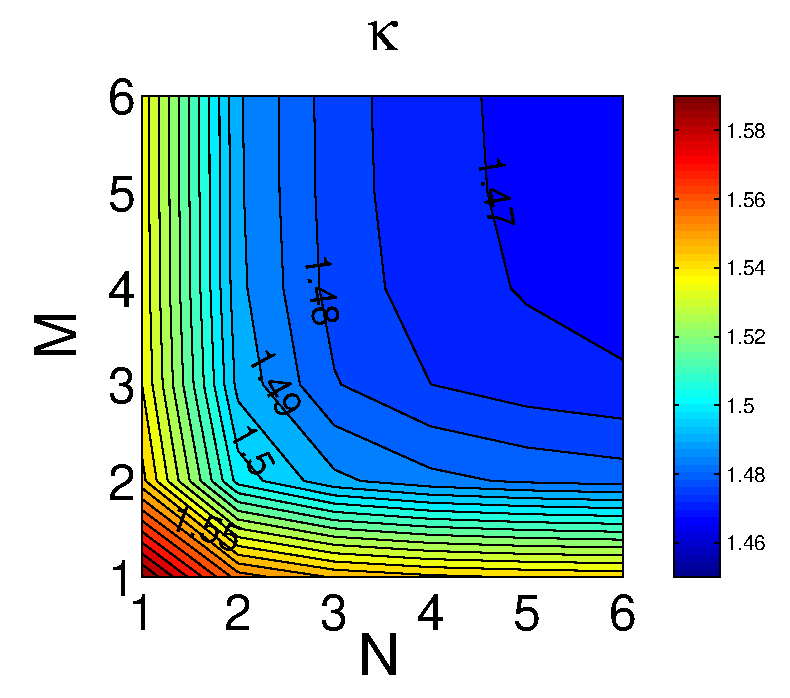
\includegraphics[width=6cm]{figures/kappa_M6_N6.eps}
\end{center}
\par
\caption{Bootstrap current coefficient $\kappa$ as a function of the highest
terms $M$ and $N$ kept in the series.}
\label{fig1}
\end{figure}

We compute the coefficient $K$ for several values of the highest terms $M$
and $N$ in the series (\ref{kappa}). The results are shown on Fig. \ref{fig1}%
. We first see that $K$ converges for high $M$ and $N$, towards a value that
seems close to 1.46. The best combination seems to be for $M=N$, as both
high $M$ and high $N$ are needed for convergence. Therefore, we take $M=N$
and calculate $K$ as a function of $M$. Results are shown on Fig. \ref{fig2}%
. We can see that $K$ indeed converges, and that the asymptotic limit is
about $K=1.46$. For $M=N=6$, we find $K=1.467$.

\begin{figure}[tbh]
\begin{center}
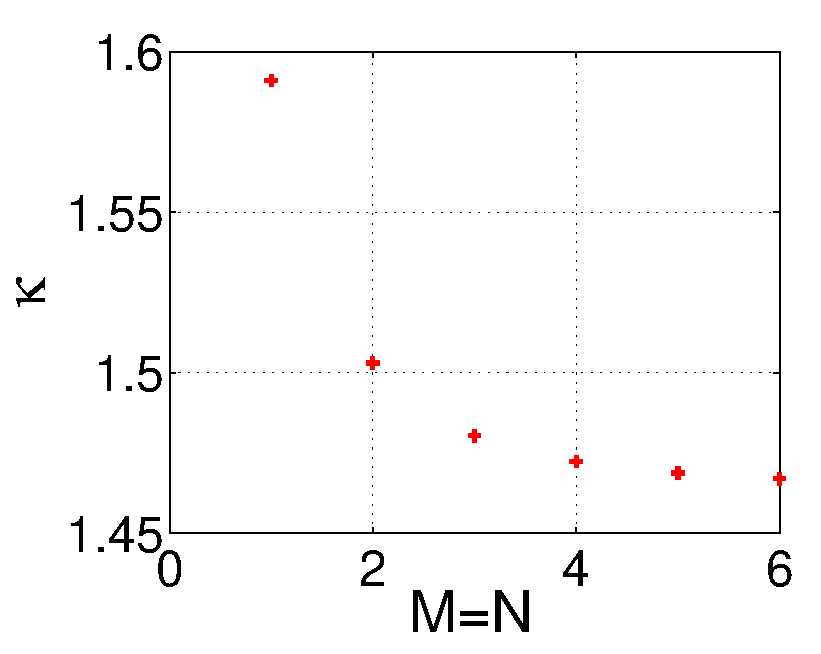
\includegraphics[width=6cm]{figures/kappa_M6.eps}
\end{center}
\par
\caption{Bootstrap current coefficient $\kappa$ as a function of the highest
terms $M$ and $N$ kept in the series, for $M=N$}
\label{fig2}
\end{figure}
